\documentclass{beamer}
\usepackage[utf8]{inputenc}
\usepackage[T1]{fontenc}
\usepackage{graphicx}
\usepackage{xcolor}
\usepackage{listings}
\usepackage{tikz}
\usetikzlibrary{positioning}
\usepackage{amsmath}
\usepackage{hyperref}

% Theme
\usetheme{Madrid}
\usecolortheme{default}

% Colors
\definecolor{codeblue}{RGB}{0,102,204}
\definecolor{codegray}{RGB}{128,128,128}
\definecolor{codegreen}{RGB}{0,128,0}
\definecolor{backcolour}{RGB}{245,245,245}

% Code listing style
\lstdefinestyle{cstyle}{
    backgroundcolor=\color{backcolour},
    commentstyle=\color{codegreen},
    keywordstyle=\color{codeblue},
    numberstyle=\tiny\color{codegray},
    stringstyle=\color{red},
    basicstyle=\ttfamily\footnotesize,
    breakatwhitespace=false,
    breaklines=true,
    keepspaces=true,
    numbers=left,
    numbersep=5pt,
    showspaces=false,
    showstringspaces=false,
    showtabs=false,
    tabsize=2,
    frame=single
}

\lstset{style=cstyle}

% Title page info
\title{Day 1: C Fundamentals and Compilation}
\subtitle{C Programming for Post-Silicon Validation Engineers}
\author{Course Instructor}
\date{6-Day Intensive Bootcamp}
\institute{Post-Silicon Validation Training Program}

\begin{document}

\frame{\titlepage}

\begin{frame}
\frametitle{Welcome to Day 1!}
\begin{center}
\Large From Zero to Validation Hero
\end{center}

\begin{itemize}
    \item \textbf{Today's Mission:} Master C basics and compilation
    \item \textbf{Validation Focus:} Chip parameter calculations
    \item \textbf{Tools:} GCC compiler, basic debugging
    \item \textbf{Outcome:} Your first validation program!
\end{itemize}

\vspace{0.5cm}
\begin{center}
\textit{"Every expert was once a beginner"}
\end{center}
\end{frame}

\begin{frame}
\frametitle{Today's Learning Objectives}
By the end of Day 1, you will:

\begin{enumerate}
    \item Understand C syntax and basic data types
    \item Write programs with variables and operators
    \item Use printf/scanf for input/output
    \item Compile programs with GCC
    \item Create validation calculations for chip parameters
    \item Handle basic compilation errors
\end{enumerate}

\vspace{0.5cm}
\begin{alertblock}{Validation Context}
All examples simulate real post-silicon validation scenarios!
\end{alertblock}
\end{frame}

\begin{frame}
\frametitle{Why C for Validation?}
\begin{columns}
\begin{column}{0.5\textwidth}
\textbf{C Advantages:}
\begin{itemize}
    \item Direct hardware access
    \item Predictable performance
    \item Minimal overhead
    \item Industry standard
    \item Embedded systems ready
\end{itemize}
\end{column}
\begin{column}{0.5\textwidth}
\textbf{Validation Needs:}
\begin{itemize}
    \item Register manipulation
    \item Timing-critical tests
    \item Memory-mapped I/O
    \item Real-time constraints
    \item Cross-platform deployment
\end{itemize}
\end{column}
\end{columns}

\vspace{0.5cm}
\begin{center}
\textbf{C = Perfect match for validation engineering!}
\end{center}
\end{frame}

\begin{frame}[fragile]
\frametitle{Your First C Program}
\begin{lstlisting}[language=C]
#include <stdio.h>

int main() {
    printf("Hello, Validation World!\n");
    return 0;
}
\end{lstlisting}

\textbf{Let's break it down:}
\begin{itemize}
    \item \texttt{\#include <stdio.h>} - Include standard I/O library
    \item \texttt{int main()} - Program entry point
    \item \texttt{printf()} - Output function
    \item \texttt{return 0;} - Success indicator
\end{itemize}
\end{frame}

\begin{frame}
\frametitle{C Data Types - The Building Blocks}
\begin{center}
\begin{tabular}{|l|l|l|l|}
\hline
\textbf{Type} & \textbf{Size} & \textbf{Range} & \textbf{Validation Use} \\
\hline
\texttt{int} & 4 bytes & $\pm 2^{31}$ & Register values \\
\texttt{float} & 4 bytes & $\pm 3.4 \times 10^{38}$ & Voltage, current \\
\texttt{char} & 1 byte & 0-255 & Status flags \\
\texttt{double} & 8 bytes & $\pm 1.7 \times 10^{308}$ & Precision timing \\
\hline
\end{tabular}
\end{center}

\vspace{0.5cm}
\begin{exampleblock}{Validation Example}
\texttt{float voltage = 3.3;} // Supply voltage\\
\texttt{int register\_value = 0x1234;} // Hardware register\\
\texttt{char status = 'P';} // Pass/Fail indicator
\end{exampleblock}
\end{frame}

\begin{frame}[fragile]
\frametitle{Variables and Declarations}
\begin{lstlisting}[language=C]
#include <stdio.h>

int main() {
    // Declare variables for chip validation
    float supply_voltage;
    int chip_id;
    char test_result;

    // Initialize values
    supply_voltage = 3.3;
    chip_id = 0x1234;
    test_result = 'P';  // P for Pass

    printf("Chip ID: 0x%X\n", chip_id);
    printf("Supply: %.1fV\n", supply_voltage);
    printf("Result: %c\n", test_result);

    return 0;
}
\end{lstlisting}
\end{frame}

\begin{frame}
\frametitle{Operators - Your Calculation Tools}
\begin{columns}
\begin{column}{0.5\textwidth}
\textbf{Arithmetic:}
\begin{itemize}
    \item \texttt{+} Addition
    \item \texttt{-} Subtraction
    \item \texttt{*} Multiplication
    \item \texttt{/} Division
    \item \texttt{\%} Modulo
\end{itemize}
\end{column}
\begin{column}{0.5\textwidth}
\textbf{Comparison:}
\begin{itemize}
    \item \texttt{==} Equal to
    \item \texttt{!=} Not equal
    \item \texttt{<} Less than
    \item \texttt{>} Greater than
    \item \texttt{<=} \texttt{>=} Less/Greater or equal
\end{itemize}
\end{column}
\end{columns}

\vspace{0.5cm}
\begin{exampleblock}{Validation Example}
\texttt{power = voltage * current;} // Calculate power\\
\texttt{if (voltage > 3.5) \{ /* overvoltage */ \}}
\end{exampleblock}
\end{frame}

\begin{frame}[fragile]
\frametitle{Input/Output with printf and scanf}
\begin{lstlisting}[language=C]
#include <stdio.h>

int main() {
    float voltage, current;

    // Get input from user (or test equipment)
    printf("Enter supply voltage (V): ");
    scanf("%f", &voltage);

    printf("Enter current (A): ");
    scanf("%f", &current);

    // Calculate and display results
    float power = voltage * current;
    printf("Power consumption: %.3f W\n", power);

    return 0;
}
\end{lstlisting}

\textbf{Format specifiers:} \texttt{\%d} (int), \texttt{\%f} (float), \texttt{\%c} (char), \texttt{\%s} (string)
\end{frame}

\begin{frame}
\frametitle{The Compilation Process}
\begin{center}
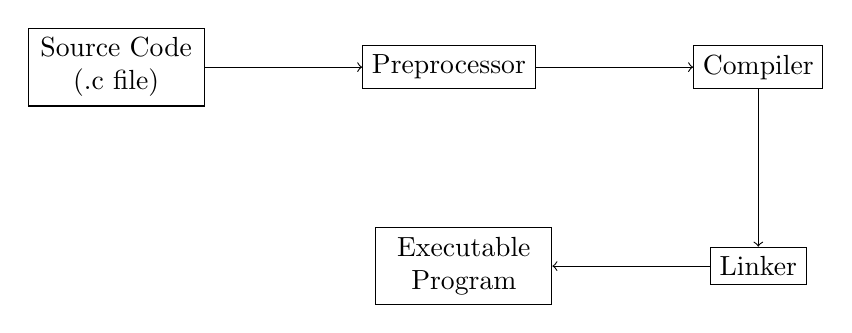
\begin{tikzpicture}[node distance=2cm]
\node (source) [draw, rectangle, text width=2cm, align=center] {Source Code\\(.c file)};
\node (preprocessor) [draw, rectangle, right=of source] {Preprocessor};
\node (compiler) [draw, rectangle, right=of preprocessor] {Compiler};
\node (linker) [draw, rectangle, below=of compiler] {Linker};
\node (executable) [draw, rectangle, left=of linker, text width=2cm, align=center] {Executable\\Program};

\draw [->] (source) -- (preprocessor);
\draw [->] (preprocessor) -- (compiler);
\draw [->] (compiler) -- (linker);
\draw [->] (linker) -- (executable);
\end{tikzpicture}
\end{center}

\textbf{GCC Command:} \texttt{gcc program.c -o program}
\begin{itemize}
    \item \texttt{-o} specifies output filename
    \item \texttt{-Wall} enables all warnings
    \item \texttt{-g} includes debugging information
\end{itemize}
\end{frame}

\begin{frame}[fragile]
\frametitle{GCC in Action}
\textbf{Compile and run:}
\begin{verbatim}
$ gcc -Wall -g voltage_check.c -o voltage_check
$ ./voltage_check
Enter supply voltage (V): 3.3
Enter current (A): 0.5
Power consumption: 1.650 W
\end{verbatim}

\textbf{Common GCC flags for validation:}
\begin{itemize}
    \item \texttt{-Wall} - Show all warnings
    \item \texttt{-g} - Include debug symbols
    \item \texttt{-O2} - Optimize for performance
    \item \texttt{-std=c11} - Use C11 standard
\end{itemize}
\end{frame}

\begin{frame}[fragile]
\frametitle{Handling Compilation Errors}
\textbf{Common errors and fixes:}

\begin{lstlisting}[language=C]
// ERROR: Missing semicolon
int voltage = 3.3  // Missing ;

// ERROR: Wrong format specifier
printf("%d", 3.14);  // Should be %f

// ERROR: Undeclared variable
printf("%f", voltge);  // Typo: should be voltage

// ERROR: Missing header
scanf("%f", &voltage);  // Need #include <stdio.h>
\end{lstlisting}

\textbf{Debugging strategy:}
\begin{enumerate}
    \item Read error messages carefully
    \item Check line numbers
    \item Look for typos and missing symbols
    \item Verify variable declarations
\end{enumerate}
\end{frame}

\begin{frame}[fragile]
\frametitle{Validation Example: Voltage Range Checker}
\begin{lstlisting}[language=C, basicstyle=\tiny]
#include <stdio.h>

int main() {
    float voltage;
    float min_voltage = 1.8;  // Minimum operating voltage
    float max_voltage = 3.6;  // Maximum safe voltage

    printf("Enter measured voltage: ");
    scanf("%f", &voltage);

    printf("Voltage: %.2fV\n", voltage);
    printf("Valid range: %.1fV - %.1fV\n", min_voltage, max_voltage);

    if (voltage < min_voltage) {
        printf("FAIL: Voltage too low!\n");
    } else if (voltage > max_voltage) {
        printf("FAIL: Voltage too high!\n");
    } else {
        printf("PASS: Voltage within range\n");
    }

    return 0;
}
\end{lstlisting}
\end{frame}

\begin{frame}
\frametitle{Interactive Poll Time!}
\begin{center}
\Large Which data type would you use for...
\end{center}

\begin{enumerate}
    \item A chip temperature reading? \pause \textcolor{green}{\textbf{float}}
    \item A 32-bit register value? \pause \textcolor{green}{\textbf{int}}
    \item A pass/fail test result? \pause \textcolor{green}{\textbf{char}}
    \item A precise timing measurement? \pause \textcolor{green}{\textbf{double}}
\end{enumerate}

\vspace{0.5cm}
\begin{center}
\textit{Think like a validation engineer!}
\end{center}
\end{frame}

\begin{frame}
\frametitle{Lab Preview: Your First Validator}
\textbf{This afternoon you'll build:}
\begin{itemize}
    \item Chip parameter validation program
    \item Input: voltage, current, temperature
    \item Processing: range checking, power calculation
    \item Output: pass/fail results with detailed feedback
    \item GitHub: commit and push your first validation code!
\end{itemize}

\vspace{0.5cm}
\textbf{Scaffolded approach:}
\begin{itemize}
    \item Starter template provided
    \item TODO comments guide implementation
    \item Pair programming encouraged
    \item TAs available for support
\end{itemize}
\end{frame}

\begin{frame}
\frametitle{Key Takeaways - Day 1}
\begin{itemize}
    \item \textbf{C is perfect for validation:} Direct, efficient, hardware-friendly
    \item \textbf{Data types matter:} Choose the right type for your measurements
    \item \textbf{GCC is your friend:} Learn the flags, read the errors
    \item \textbf{Start simple:} Basic I/O and calculations are powerful
    \item \textbf{Think validation:} Every program can simulate real testing
\end{itemize}

\vspace{0.5cm}
\begin{center}
\textbf{You're already thinking like a validation engineer!}
\end{center}
\end{frame}

\begin{frame}
\frametitle{Tonight's Homework}
\textbf{Extend your validator program:}
\begin{enumerate}
    \item Add error handling for invalid inputs
    \item Include more validation parameters
    \item Improve user interface with better prompts
    \item Document your code with comments
    \item Submit via GitHub pull request
\end{enumerate}

\vspace{0.5cm}
\textbf{Reading:}
\begin{itemize}
    \item Review today's code examples
    \item Preview tomorrow's control flow concepts
    \item Explore GCC documentation
\end{itemize}
\end{frame}

\begin{frame}
\frametitle{Questions \& Discussion}
\begin{center}
\Large Let's discuss!
\end{center}

\begin{itemize}
    \item What validation scenarios can you imagine?
    \item Which concepts need more clarification?
    \item How does this relate to your current work?
    \item Any compilation issues to troubleshoot?
\end{itemize}

\vspace{1cm}
\begin{center}
\textbf{Ready for hands-on lab time!}
\end{center}
\end{frame}

\end{document}

